\chapter{Parallelism}

% Brett
\section{Flat Parallelism}
When the project started, the version of Kokkos installed on our machine did not include teams. That meant that we could not use any algorithms that required shared memory or reductions. We had access to an atomic fetch and add function, but this can cause a huge bottleneck in programs if too many threads are trying to write to the same memory location. This meant we were limited to writing algorithms in which each thread knew its responsibility and did not have to worry about race conditions, in other words it did not interact with other threads in any capacity. In this section we will describe how to write high performing kernels for both the CPU and GPU using this flat parallelism technique. We will also describe some of its shortcomings and which other non-flat parallel algorithms can help fix these shortcomings.

The main factors that greatly effect performance are the thread count, a thread's responsibility, access patterns, and how data is laid out in memory. The first two of which are all linked together and directly effect each other. Figuring out what the thread count for a given problem should be is typically done by breaking down the problem into smaller pieces and calculating how many smaller pieces there are. For example, in ContractFieldFieldScalar, which is many matrix multiplications, it is easy to make one thread do one matrix multiplication meaning the thread count must be equal to the number of cells, or matrix multiplications, that must be calculated. Figuring out the best way to break down the responsibility of a single thread requires looking at the expected problem size. Since the average use case for the example of ContractFieldFieldScalar is one thousand to tens of thousands of cells, with matrix sizes around 
eight by eight or sixty-four by one hundred twenty-five, it is best to break down the problem into the smallest possible pieces. This is because creating a thread for every cell is ill-advised because that means as little as one thousand threads may be created, which is nowhere near saturating the GPU, which means we want many threads to calculate a single matrix multiplication. Since the one thousand to a couple tens of thousands of cells is the expected use case for all of the contraction problems, the idea of wanting many threads per contraction holds true for all of them. 

The question now is: how many threads per contraction is optimal? Well, looking at our thread count, which is going to be a couple thousand multiplied by the number of threads per contraction, it is best to have anywhere between a couple hundred to a thousand. This will ensure that the GPU is being saturated and the most parallelism is taking place, meaning higher performance. However, the limitation of the threads not being able to interact or write to the same memory location means the most threads per contraction is equal to the number of entries in the output tensor. Looking at our problem size again, the expected output tensor dimensions range from a single number (for any problem that contains DataData in its name), to sixty-four squared (biggest values for numLeftFields and numRightFields which are the dimensions of the output matrix for some problems). This range is smaller than the couple hundred to a thousand that we were hoping for, which means it is best to create a thread per output element per contraction. The thread count and it's responsibility are now known and optimized for our problem sizes. The logic may vary depending on problem size and dimensions, but the goal of saturating the GPU is always the priority.

Now that the number of threads and their responsibility are known, the best access patterns and data layout must be calculated. As described earlier, the best access patterns and data layouts for threads on the CPU are ones that utilize the cache. This means that for the CPU, or when using Kokkos::OpenMP, we want a thread's next memory read to be next to its current memory read. However, on the GPU, or when using Kokkos::Cuda, a thread's memory read should be next to the memory read of the thread right next to it. These two optimizations directly conflict, but lucky for us, Kokkos' View data structure has two layouts, LayoutLeft and LayoutRight, which changes how data is laid out in memory. This means we can use LayoutLeft for one architecture, say Kokkos::Cuda, and LayoutRight for the other, Kokkos::OpenMP. So the trick is figuring out how to arrange the data, or which order to put the indices so that one layout coalesces the memory while the other uses the cache. This is best shown by an example, in ContractFieldFieldScalar there are inputs $A_{c, l, p}$ and $B_{c, r, p}$. Assuming we have a thread per output element in output $C_{c, l, r}$, then we can have the inputs ordered as follows: $A_{c, l, p}$ and $B_{c, r, p}$. When using Kokkos::OpenMP, the Views will be LayoutRight, so $A_{i, j, k}$ will be right next to $A_{i, j, k+1}$ in memory, while $A_{i, j, k}$ will be very far from $A_{i+1, j, k}$ in memory. Each thread needs to do a dot product of a row in $A$ with a column in $B$, so a thread needs to loop through all of $p$ for the same value of $c$ and $l$ in $A$ and also loop through all of $p$ for the same $c$ and $r$ in $B$. Notice however that all the different value of $p$ in $A$ and $B$, where $c$, $l$, and $r$ are fixed, are next to each other in memory. This means that it will be cache friendly for any thread. 

Now looking at Kokkos::Cuda which is using a LayoutLeft View, the memory needs to be coalesced to be optimal. Thus, to get the best performance the algorithm needs to be smart about the work that a thread does relative to other nearby threads. Since $c$ values that differ by 1 are next to each other in memory (because LayoutLeft is being used now), it is best to have thread $x+1$ to do the same work as thread $x$, but for the next cell. For example, thread $x$ is responsible for calculating $C_{i, j, k}$ so thread $x+1$ is responsible for calculating $C_{i+1, j, k}$,. This way the memory is always coalesced. 

Finding the best way to layout memory to optimize for both the CPU and GPU is not too difficult. One technique is to first find the best way for caching, then imagine using the opposite layout (left or right) and seeing if there is any way to coalesce the memory. This way one functor can be used, the data layout can be easily changed, and the performance for both the CPU and GPU will be high. Using this flat parallel technique we have received many good results, an example of which can be seen in Figure~\ref{lst:ContractFieldFieldScalar speedup over serial}, but there are some issues with flat parallelism.

\begin{figure}[!ht]
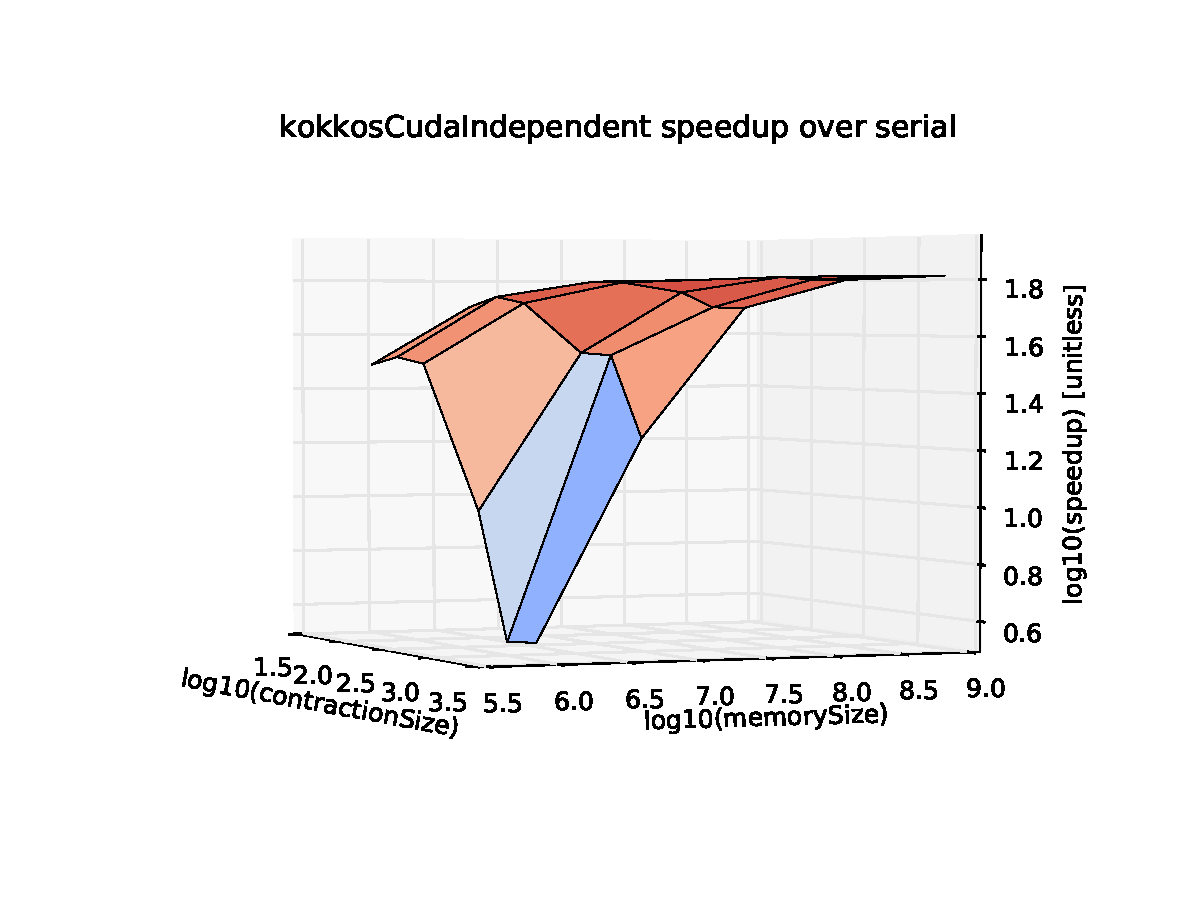
\includegraphics[scale=.8]{CFFS_VersusSerial_kokkosCudaIndependent.pdf}
\caption{Speedup over serial of the flat parallel algorithm of the ContractFieldFieldScalar kernel. At its best this algorithm runs 60 times faster than serial. The closest corner, where speedup is only about 4 times, does not fit into Sandia's use case of expected problem sizes.
\label{lst:ContractFieldFieldScalar speedup over serial}} 
\end{figure}

The biggest issue with the flat parallelism technique is that there isn't always enough parallelism for the GPU. For all the problems that have DataData in the name, the output is simply an array of numbers, meaning that only one thread per contraction can be used. The GPU is great for using tens of thousands of threads to do computation, but when the number of threads is severely limited, the CPU performs much better. For some of our problems, there are test runs where serial CPU code out performed the same problem running on the GPU. This is a scenario that should not happen for these types of problems. The issue is that a small number of threads were created, but there was a lot of work that the thread needed to do. Since CPU's are much faster when comparing a single thread to a single thread on the GPU, it is no surprise the CPU outperforms the GPU in this situation. However to fix it, a thread's job needs to be split up between more threads. As mentioned earlier, this is not allowed in flat parallelism because the threads would need to a mechanism to avoid race conditions when writing to the same location. This is where the reduction method that is described in the next section becomes useful.

Another feature of the GPU that can be leveraged, that is not the flat parallel scope, is shared memory. Shared memory is essentially a user controlled cache on the GPU. Algorithms that use shared memeory will be discussed in Section~\ref{slicing} and Section~\ref{sec:tiling}. The main benefits of not using shared memory are it is easier to code and the speedup of shared memory is relatively small compared to the speedup flat parallel algorithms reap over serial code. 

% Ellen
\section{Reduction} \label{sec:reduction}
In some cases, flat parallelism can perform very poorly.  One problem with flat
parallelism is the potential lack of enough parallelism, as in
\texttt{ContractDataDataTensor}.  \texttt{ContractDataDataTensor} takes two
input arrays of three-dimensional tensors and produces an array of scalars.  See
Section~\ref{section:ContractDataDataTensor} for a more complete description of
this kernel.

The problem with the \texttt{DataData} class of tensor contractions (see
Table~\ref{tab:IntrepidNamingConvention}) is that they all output an array of
scalars -- that is, each individual contraction produces a scalar output.
Therefore, using flat parallelism, the greatest number of threads we can spawn
is one thread per contraction.  Each thread must then perform an entire
contraction independently, which in the case of \texttt{ContractDataDataTensor},
means looping over all three of the contraction indices.

Because of this, we see that when the contraction size is large and the memory size is
small -- when we cannot spawn enough threads to saturate the GPU and each thread
is responsible for a large amount of computation --
\texttt{ContractDataDataTensor} actually performs worse than serial.

A solution to this problem is to use a parallel reduction algorithm instead of a
flat parallelism algorithm.  In a reduction, multiple threads contribute to a
single output element.  This adds the necessary overhead of coordinating between
threads and combining their contributions.

In Kokkos, threads can be organized into teams, which correspond to Cuda blocks.
Built-in reduction methods allow teams to merge the contributions of its
constituent threads.

Using this team-thread paradigm, we explored several methods of implementing
\texttt{ContractDataDataTensor} using a reduction algorithm.

\subsection{Team Depth 1}
    In this reduction algorithm, we assign one team per contraction, and each
    team has as many threads as there are elements in the \texttt{iVec2}
    dimension.  Each thread therefore performs $\texttt{numPoints} \times
    \texttt{iVec1}$ multiplications, and then combines its local sum with that
    of the other threads in the team.


\begin{figure}[ht]
    \begin{lstlisting}
    // A team does one cell
    const unsigned int cellIndex = thread.league_rank();

    float sum = 0;
    // Each of the _dim1 threads contracts the qp and d1 dimensions
    Kokkos::parallel_reduce(Kokkos::TeamThreadLoop(thread, _dim2),
        [&] (const unsigned int dim2, float& localsum) {
          for (unsigned int qp=0; qp < _numPoints; ++qp) {
            for (unsigned int d1=0; d1 < _dim1; ++d1) {
              localsum +=  _leftInput(cellIndex, qp, d1, dim2) *
                _rightInput(cellIndex, qp, d1, dim2);
            }
          }
      }, sum);

    if (thread.team_rank() == 0) {
      _output(cellIndex) = sum;
    }
 \end{lstlisting}
\caption{Code from Team Depth 1 reduction functor for \texttt{ContractDataDataTensor}
\label{lst:ContractDataDataTensorDepth1Functor}} 
\end{figure}

\begin{figure}[ht]
    \begin{lstlisting}
    const team_policy reduction_policy(numCells, iVec2);
    Kokkos::parallel_for(reduction_policy, contractDataDataTensorTeamDepth1Functor );
    Kokkos::fence();
 \end{lstlisting}
\caption{Code from kernel launch for \texttt{ContractDataDataTensor} Team Depth
1 reduction
\label{lst:ContractDataDataTensorDepth1Call}} 
\end{figure}

In Figure~\ref{lst:ContractDataDataTensorDepth1Functor}, we can see that each
thread loops over the \texttt{numPoints} and \texttt{iVec1} dimensions, and then
reduces with the other threads in the team.  The call to Kokkos'
\texttt{parallel\_for} function, seen in
Figure~\ref{lst:ContractDataDataTensorDepth1Call}, specifies an execution policy
in which the number of teams launched is \texttt{numCells}, and each team has
\texttt{iVec1} threads.

\begin{figure}[ht]
    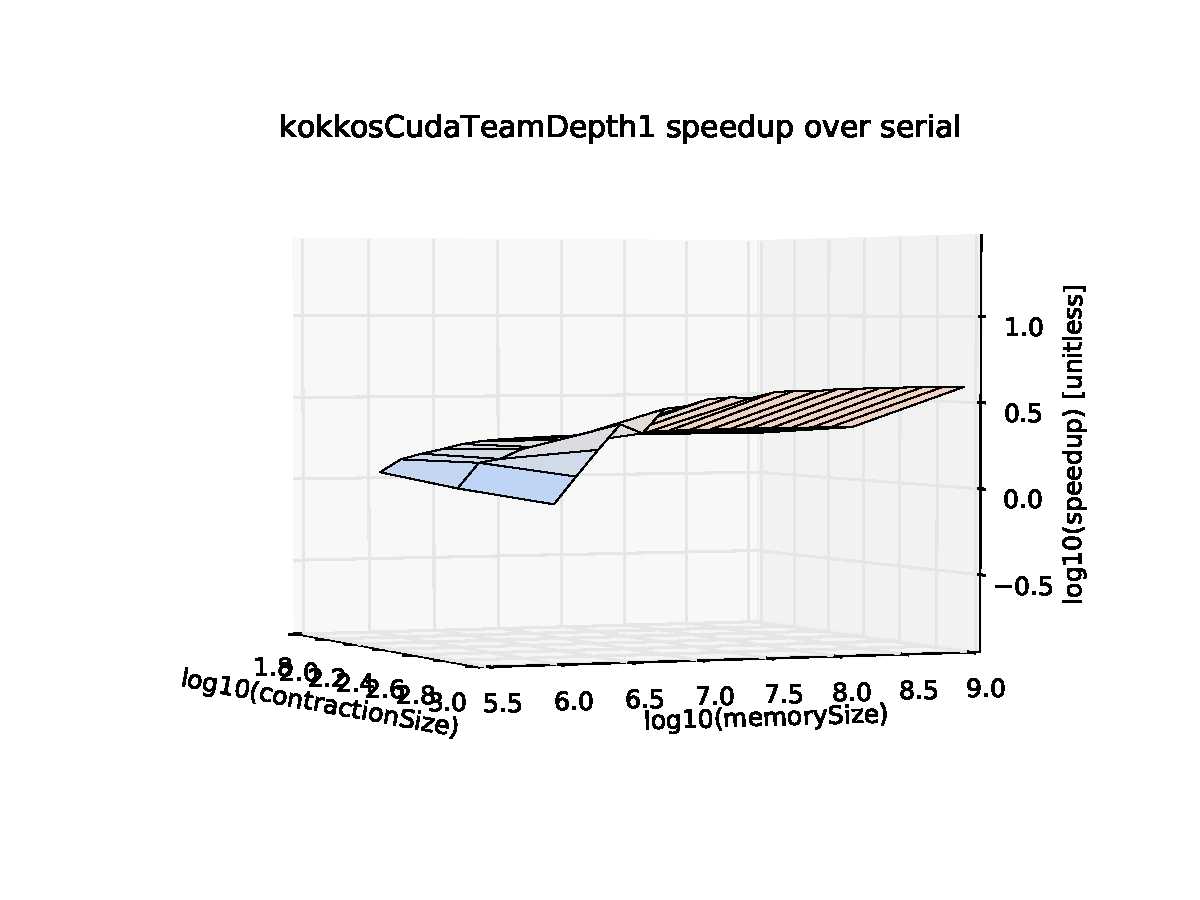
\includegraphics[scale=.55]{./VersusSerial_kokkosCudaTeamDepth1_clearCache_shadowfax.pdf}
\caption{Speedup of ContractDataDataTensor with Team Depth 1 algorithm over
    serial
\label{fig:ContractDataDataTensorDepth1}} 
\end{figure}

As shown in Figure~\ref{fig:ContractDataDataTensorDepth1}, this Team Depth 1
algorithm performs generally better than serial, but the speedup is minimal.
Therefore, we explored other reduction algorithms, which we hoped would yield
more impressive results.

\subsection{Team Depth 2}
    This reduction algorithm is similar to the previous one.  As with the Team
    Depth 1 reduction, we assign one team per contraction.  Each team has
    $\texttt{iVec1} \times \texttt{iVec2}$ threads, each responsible for
    \texttt{numPoints} multiplications.  Each thread then combines its local sum
    with that of the other threads in the team.

\begin{figure}[ht]
    \begin{lstlisting}
    // A team does one cell
    const unsigned int cellIndex = thread.league_rank();

    float sum = 0;
    // Each of the _dim1 * _dim2 threads qp dimension
    Kokkos::parallel_reduce(Kokkos::TeamThreadLoop(thread, _dim1 * _dim2),
        [&] (const unsigned int threadIndex, float& localsum) {
          const unsigned int dim1 = threadIndex / _dim2;
          const unsigned int dim2 = threadIndex % _dim2;

          for (unsigned int qp = 0; qp < _numPoints; ++qp) {
            localsum +=  _leftInput(cellIndex, qp, dim1, dim2) *
              _rightInput(cellIndex, qp, dim1, dim2);
          }

      }, sum);

    if (thread.team_rank() == 0) {
      _output(cellIndex) = sum;
    }
    
 \end{lstlisting}
\caption{Code from Team Depth 2 reduction functor for \texttt{ContractDataDataTensor}
\label{lst:ContractDataDataTensorDepth2Functor}} 
\end{figure}

\begin{figure}[ht]
    \begin{lstlisting}
    const team_policy reduction_policy(numCells, iVec2 * iVec1);
    Kokkos::parallel_for(reduction_policy, contractDataDataTensorTeamDepth2Functor );
    Kokkos::fence();
 \end{lstlisting}
\caption{Code from kernel launch for \texttt{ContractDataDataTensor} Team Depth
2 reduction
\label{lst:ContractDataDataTensorDepth2Call}} 
\end{figure}

In Figure~\ref{lst:ContractDataDataTensorDepth2Functor}, we can see that each
thread loops over the \texttt{numPoints} dimension only, and then
reduces with the other threads in the team.  The call to Kokkos'
\texttt{parallel\_for} function, seen in
Figure~\ref{lst:ContractDataDataTensorDepth2Call}, specifies an execution policy
in which the number of teams launched is \texttt{numCells}, and each team has
$\texttt{iVec1}\times\texttt{iVec2}$ threads.

\begin{figure}[ht]
    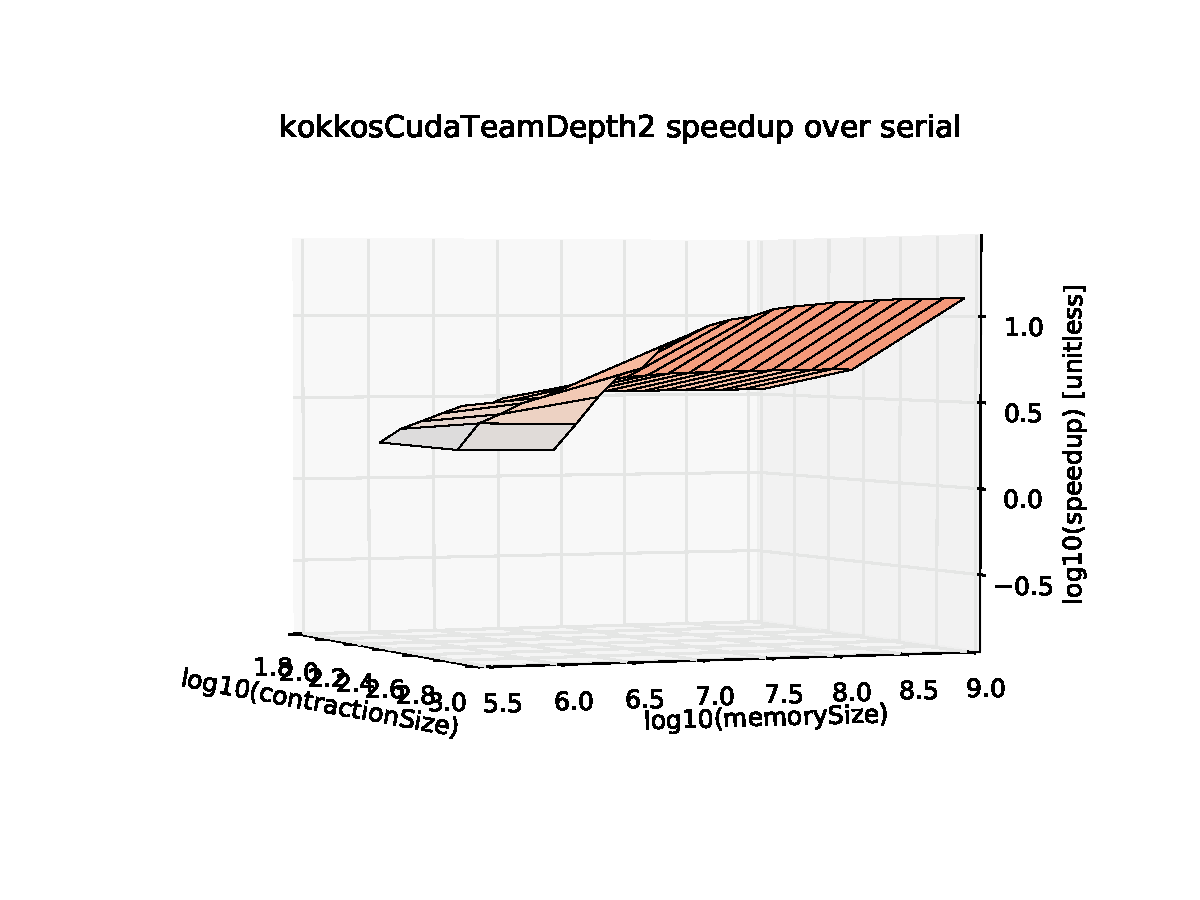
\includegraphics[scale=.55]{./VersusSerial_kokkosCudaTeamDepth2_clearCache_shadowfax.pdf}
\caption{Speedup of ContractDataDataTensor with Team Depth 2 algorithm over
    serial
\label{fig:ContractDataDataTensorDepth2}} 
\end{figure}

As shown in Figure~\ref{fig:ContractDataDataTensorDepth2}, this Team Depth 2
algorithm always performs better than serial.  In addition, the speedup is
significant, and for large memory sizes, performs nearly as well as the flat
parallel algorithm.  Given the necessary overhead of performing a reduction, we
believe this to be a fairly good algorithm for good performance across the
board.

However, because the team size is fixed based on the size of the \texttt{iVec1}
and \texttt{iVec2} dimensions, this algorithm may suffer performance penalties
or perhaps even bugs if these two dimensions are of unexpected sizes.  A more
generalizable algorithm therefore would be preferable.

\subsection{Teamstride}
    A more robust algorithm is one we call the Teamstride algorithm, in which
    each contraction is still assigned to a team, but a fixed number of threads
    are spawned for each team.  These threads treat the three contraction
    indices (\texttt{numPoints}, \texttt{iVec1}, \texttt{iVec2}) as if they were
    a single index, each thread striding forwards by the number of threads on
    this ``combined'' index.  For instance, if this algorithm were run with a
    team size of sixty-four threads, then the zeroth thread in a team would sum
    the product of the zeroth elements, the sixty-fourth, the 128th, and so on.
    
\begin{figure}[ht]
    \begin{lstlisting} [basicstyle=\tiny]
    // A team does one cell
    const unsigned int cellIndex = thread.league_rank();

    // Some useful derived constants that we'll reuse
    const unsigned int dim12 = _dim1 * _dim2;
    const unsigned int cellSize = _numPoints * dim12;

    float sum = 0;

    Kokkos::parallel_reduce
      (Kokkos::TeamThreadLoop(thread,cellSize),
       [&](const unsigned int indexWithinContraction, float & localsum) {

        // Calculate the next element to add (striding by teamsize)
        const unsigned int qp = indexWithinContraction / dim12;
        const unsigned int indexWithinTens1Tens2Thing =
          indexWithinContraction - qp * dim12;
        const unsigned int iTens1 = indexWithinTens1Tens2Thing / _dim2;
        const unsigned int iTens2 = indexWithinTens1Tens2Thing - iTens1*_dim2;

        localsum +=  _leftInput(cellIndex, qp, iTens1, iTens2) *
          _rightInput(cellIndex, qp, iTens1, iTens2);
      } , sum );

    if (thread.team_rank() == 0) {
      _output(cellIndex) = sum;
    }
    \end{lstlisting}

\caption{Code from Teamstride functor for \texttt{ContractDataDataTensor}
\label{lst:ContractDataDataTensorTeamstrideFunctor}} 
\end{figure}

\begin{figure}[ht]
    \begin{lstlisting}[basicstyle=\tiny]
    const team_policy reduction_policy(numCells, 32);
    Kokkos::parallel_for( reduction_policy, contractDataDataTensorTeamstrideFunctor );
    Kokkos::fence();
    \end{lstlisting}
\caption{Code from kernel launch for \texttt{ContractDataDataTensor} Teamstride
\label{lst:ContractDataDataTensorTeamstrideCall}} 
\end{figure}

As seen in Figure~\ref{lst:ContractDataDataTensorTeamstrideFunctor}, this
algorithm requires more arithmetic on the part of each thread, and the thread
is not responsible for looping over a single subset of indices, instead looping
over all three contraction indices. The corresponding call in
Figure~\ref{lst:ContractDataDataTensorTeamstrideCall} uses a fixed team size of
32, unlike the previous two algorithms.

\begin{figure}[ht]
    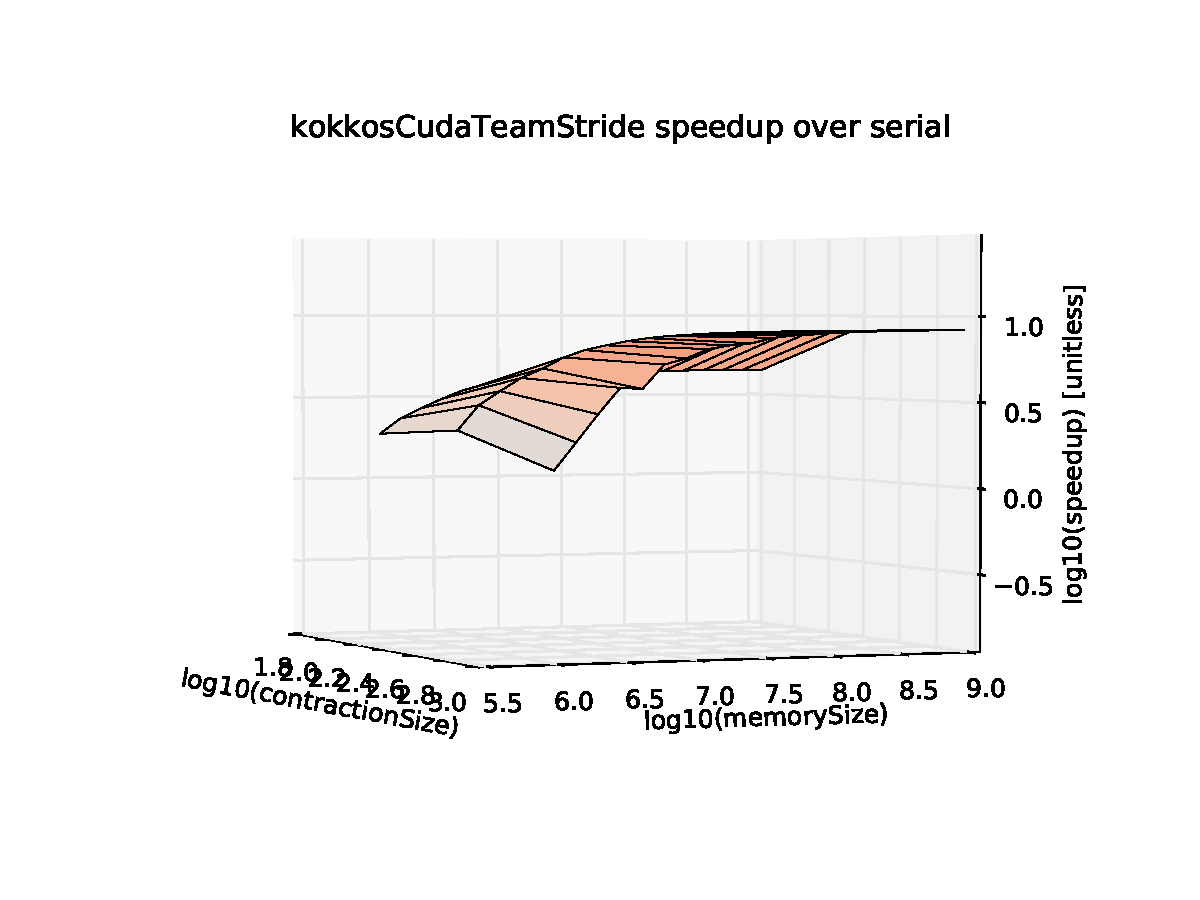
\includegraphics[scale=.55]{./VersusSerial_kokkosCudaTeamStride_clearCache_shadowfax.pdf}
\caption{Speedup of ContractDataDataTensor with Teamstride algorithm over
    serial
\label{fig:ContractDataDataTensorTeamstride}} 
\end{figure}

As shown in Figure~\ref{fig:ContractDataDataTensorTeamstride}, this algorithm
always performs better than serial.  Like with Team Depth 2, the speedup is
significant, and for large memory sizes, performs nearly as well as the flat
parallel algorithm.  In addition, this algorithm is more robust than Team Depth
2, since the number of threads per team is not determined by the size of the
input dimensions.  Therefore, the Teamstride reduction algorithm is likely the
most generalizable and performant variant of the reduction algorithms, and
should be explored in tensor contraction functions in which the inputs may
consist of a few large tensor contractions.

\subsection{Reduction Special Case}
As mentioned above, the parallel reduction algorithm performs best when in the flat parallel algorithm there is a small number of threads but lots of work per thread. However, we created parallel reduction algorithms for problems that did not have this problem such as ContractFieldFieldScalar which could have as small as eight multiplies for a single thread since $p$ could be as small as 8. As one may guess, this algorithm performs much worse than the flat parallel algorithm. This is because we are creating more threads than necessary and dividing up a small amount of work between at least 32 threads. The work is divided between at least 32 threads because, remembering the architecture of the GPU, there are 32 threads in a warp all of which run in lock step. So in cases where $p < 32$ threads are created that are not used in this reduction algorithm. To mitigate this phenomenon we created a special reduction case.

The special reduction case creates less teams, giving more work per team, if more than half of the threads are being wasted. This means in the case of ContractFieldFieldScalar where 24 threads are wasted, because only 8 need to do the multiply and reduction, one quarter of the teams are created, and each team is responsible for calculating four times as many outputs elements. This case adds the following code in the functor's operator() function: \\
\begin{figure}[!ht]
    \begin{lstlisting}
if (numPoints <= 16) {	
	int myID = thread.league_rank()*(threadsPerTeam/numPoints)+thread.team_rank()/numPoints;
	int myMatrix = myID / (numLeftFields * numRightFields);
	int matrixIndex = myID - (myMatrix * (numLeftFields * numRightFields));
	int matrixRow = matrixIndex / numRightFields;
	int matrixCol = matrixIndex - (matrixRow * numRightFields);

	int pointIndex = thread.team_rank() % numPoints;

	float mult = leftView(myMatrix, matrixRow, pointIndex) 
		* rightView(myMatrix, pointIndex, matrixCol);

	Kokkos::atomic_fetch_add(&outputView(myMatrix, matrixRow, matrixCol), mult);
}
    \end{lstlisting}
\caption{Code for the special reduction case in \texttt{ContractFieldFieldScalar}
\label{lst:ContractFieldFieldScalarReductionSpecialCase}} 
\end{figure}

In the code above if the number of multiplies, which is numPoints for this kernel, is less than 16 then we want one team to do more than one output. This reduces the total number of wasted threads meaning more efficiency and speed. One thing that needs to be noted for the code in the special case is that an atomic\_fetch\_add is used instead of a team reduce. This is due to the fact that there is no team\_reduce function where half the threads reduce to one location while the other half reduce to another location. This has the side effect of requiring the output locations to be 0 before the calculation, while in the "normal" reduction algorithm that is not necessary. 

Another point that needs to be reiterated is that this special case performs worse than the flat parallel algorithm, but its purpose is to increase the performance of a pure reduction algorithm. Here are the graphs that show the effect of using this special case. 

\begin{figure}[!ht]
    \centering
    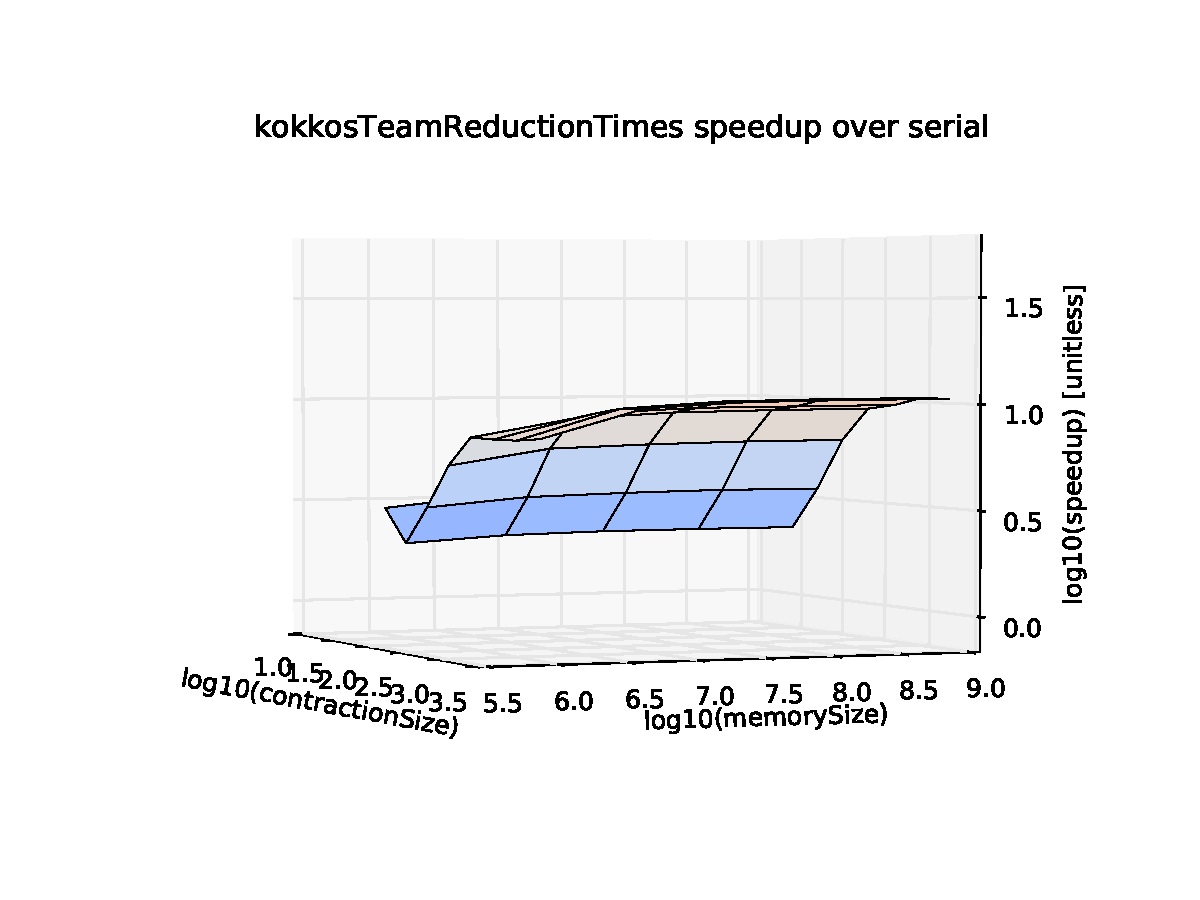
\includegraphics[scale = .8]{kokkosCFFSTeamReductionSpecialCase.pdf}
    \caption{Here is a graph showing the special case of Team Reduction algorithm's speedup over serial for ContractFieldFieldScalar. The faster speeds for the smaller contraction size (far left) is where the special case is used. }
\end{figure}

Compare this to the graph of the same exact team reduction without the special if case. Notice that the flap on for small contraction sizes does not exist and is much smaller than the speeds of the same contraction size using the special case.

\begin{figure}[!ht]
    \centering
    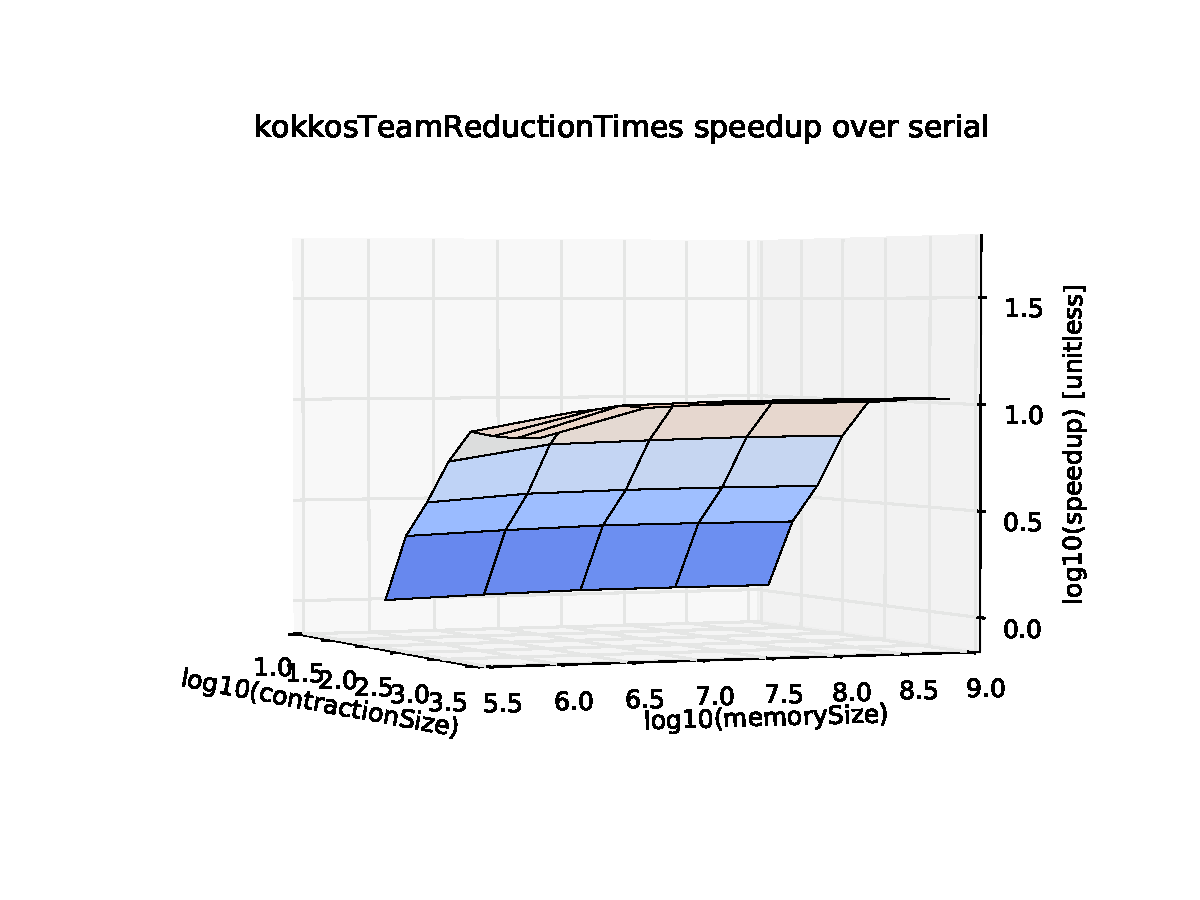
\includegraphics[scale = .8]{kokkosCFFSTeamReductionNoSpecialCase}
    \caption{ContractFieldFieldScalar team reduction's speedup over serial without the special case in the reduction. Notice that the smaller contraction sizes continue to perform worse, which was not the case for the reduction algorithm with the special case.}
\end{figure}

Overall, the special case of having one team calculate multiple outputs in order to use up all of its threads is worse than the speedup of the flat parallel algorithm. This is just mentioned because we wanted to make sure our reduction algorithm was performing as high as possible. 

% Alex
\section{Slicing} \label{slicing}
Another general method we used for these contractions was Slicing. The first step of this method was to load one full contraction from the left matrix into shared memory. Then, we simultaneously computed every output element that was dependent on that contraction as input. The clearest way to explain the algorithm is by example. Consider one of the matrix multiplications in ContractFieldFieldScalar. 

\begin{figure}
    \centering
    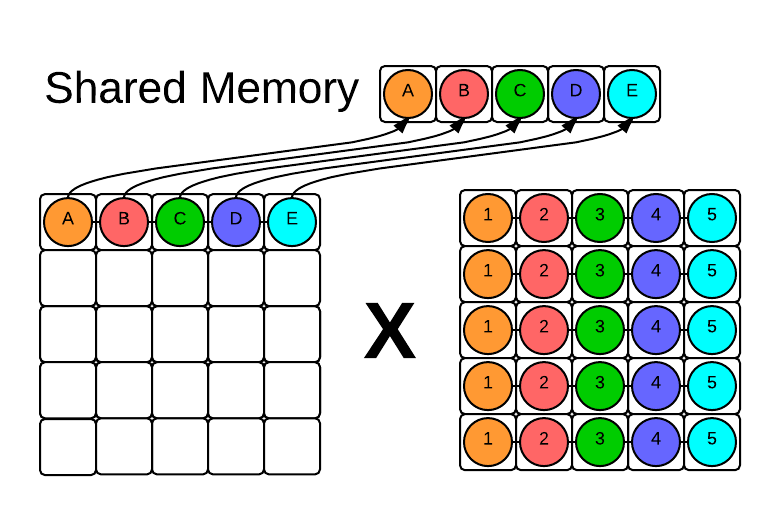
\includegraphics[scale = .55]{ContractFieldFieldScalarGraphic}
    \caption{Demonstration of memory accesses for a slicing implementation of ContractFieldFieldScalar}
\end{figure}

	On the left, we have the first of the two input matrixes, who's first row elements are labeled $A-E$. On the right we have the second of the two inputs. For the sake of simplicity, assume that we have on block of five threads which are labeled by color. Each of the threads reads in one of the elements on the right and copies it into shared memory. In cases where the number of elements per contraction (row on the left) is unequal to the number of contractions (columns on the right), we set the number of threads per block equal to the number of contractions. This causes threads to either sit idle or loop multiple times when reading the elements on the left into shared memory, but this is clearly more efficient than forcing threads to compute more than one element.
	
	After the values of the contraction have been read into shared memory, we have each thread compute the output element corresponding to one contraction. This is shown on the right by the colored columns. Each thread reads every element from shared memory and computes the contraction by multiplying these elements with the columns of the right matrix. We see that throughout this progress, memory accesses will be coalesced within the block, since each thread reads the same element from shared memory then multiplies by an element that is adjacent to the other elements the rest of the block is reading at that time. 
	
	For every other block of threads, the approach is similar, if Figure 3.1 represents the first block of the contraction, then the second block will be represented as below. 

\begin{figure}[b]
    \centering
    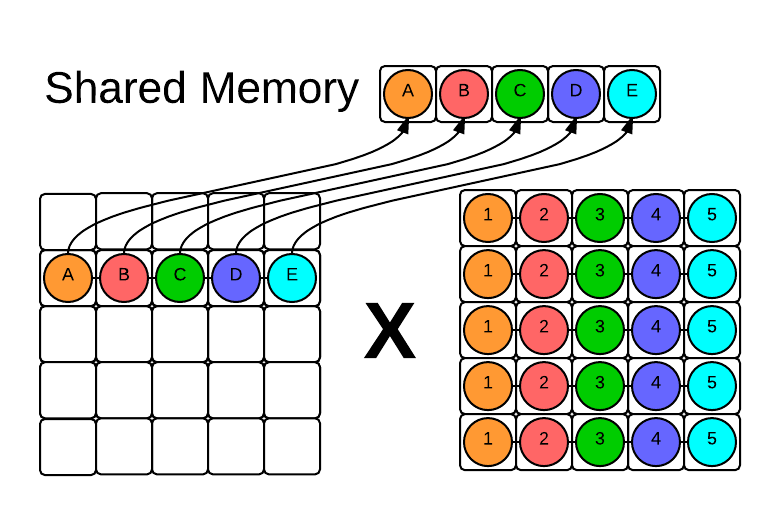
\includegraphics[scale = .55]{ContractFieldFieldScalarGraphic2}
    \caption{Demonstration of memory accesses for the second block of a slicing implementation of ContractFieldFieldScalar}
\end{figure}

We see that for the FieldFieldScalar example, where our equation is given by $L_{C,\ell,P} \times R_{C, \mathcal{R}, P} = O_{C,\ell, \mathcal{R}}$, the number of blocks initialized by the algorithm will be equal $\ell \times C$, since there are $\ell$ blocks per matrix, and we have $C$ matrices. Additionally, there will be $\mathcal{R}$ threads per block. 

	Code for executing the algorithm as described above is included below, although it has been simplified for clarity. 

\begin{figure}[ht]
    \begin{lstlisting} [basicstyle=\tiny]
     extern __shared__ float sliceStorage[];
     const unsigned int col = threadIdx.x;
     unsigned int currentBlock = blockIdx.x;
     unsigned int numBlocks = numBasis*numCells;
     
     syncthreads();
     const unsigned int cell = currentBlock / numBasis;
     const unsigned int row = currentBlock - cell * numBasis;

     for (unsigned int p = threadIdx.x; p < contractionSize; p += blockDim.x) {
        sliceStorage[p] = dev_contractionData_Left[cell*numBasis*contractionSize + row*contractionSize + p];
     }
     syncthreads();

     float sum = 0;
     for (int p = 0; p < contractionSize; ++p) {
       sum += sliceStorage[p] * dev_contractionData_Right[cell*numBasis*contractionSize +
        p*numBasis + col];
     }

     dev_contractionResults[cell*numBasis*numBasis + row*numBasis + col] = sum;
 \end{lstlisting}
\caption{Code from slicing algorithm on \texttt{ContractFieldFieldScalar}
\label{lst:ContractFieldFieldScalarSlice}} 
\end{figure}

	The main advantage of this approach is that it is easily generalizable to tensor contractions of higher dimensions. Unlike tiling, which is significantly less intuitive in higher dimensions, it is easy to implement slicing in higher dimensions by loading a larger slice into shared memory. Because of its reliance on shared memory, there are many use cases in which we would expect slicing to perform poorly. Intuitively, slicing is reliant on large contraction sizes to produce speedup because in situations where the number of threads per block is low it is unable to saturate the GPU. While this problem can be remedied by increasing the number of contractions per block, it can introduce problems with shared memory. Since shared memory is limited by nature, slicing has to balance the amount of work per block with the amount of shared memory available to that block.
	
	In situations where the problem has an inherently large amount of reuse like ContractFieldFieldScalar, this problem can be remedied to some degree, but in contractions without this feature, like ContractDataDataScalar, it seems clear that slicing will not be an efficient algorithm. 
	
When we compare slicing approaches using one contraction per block to independent flat parallelism on promising problems, we get underwhelming results. 

    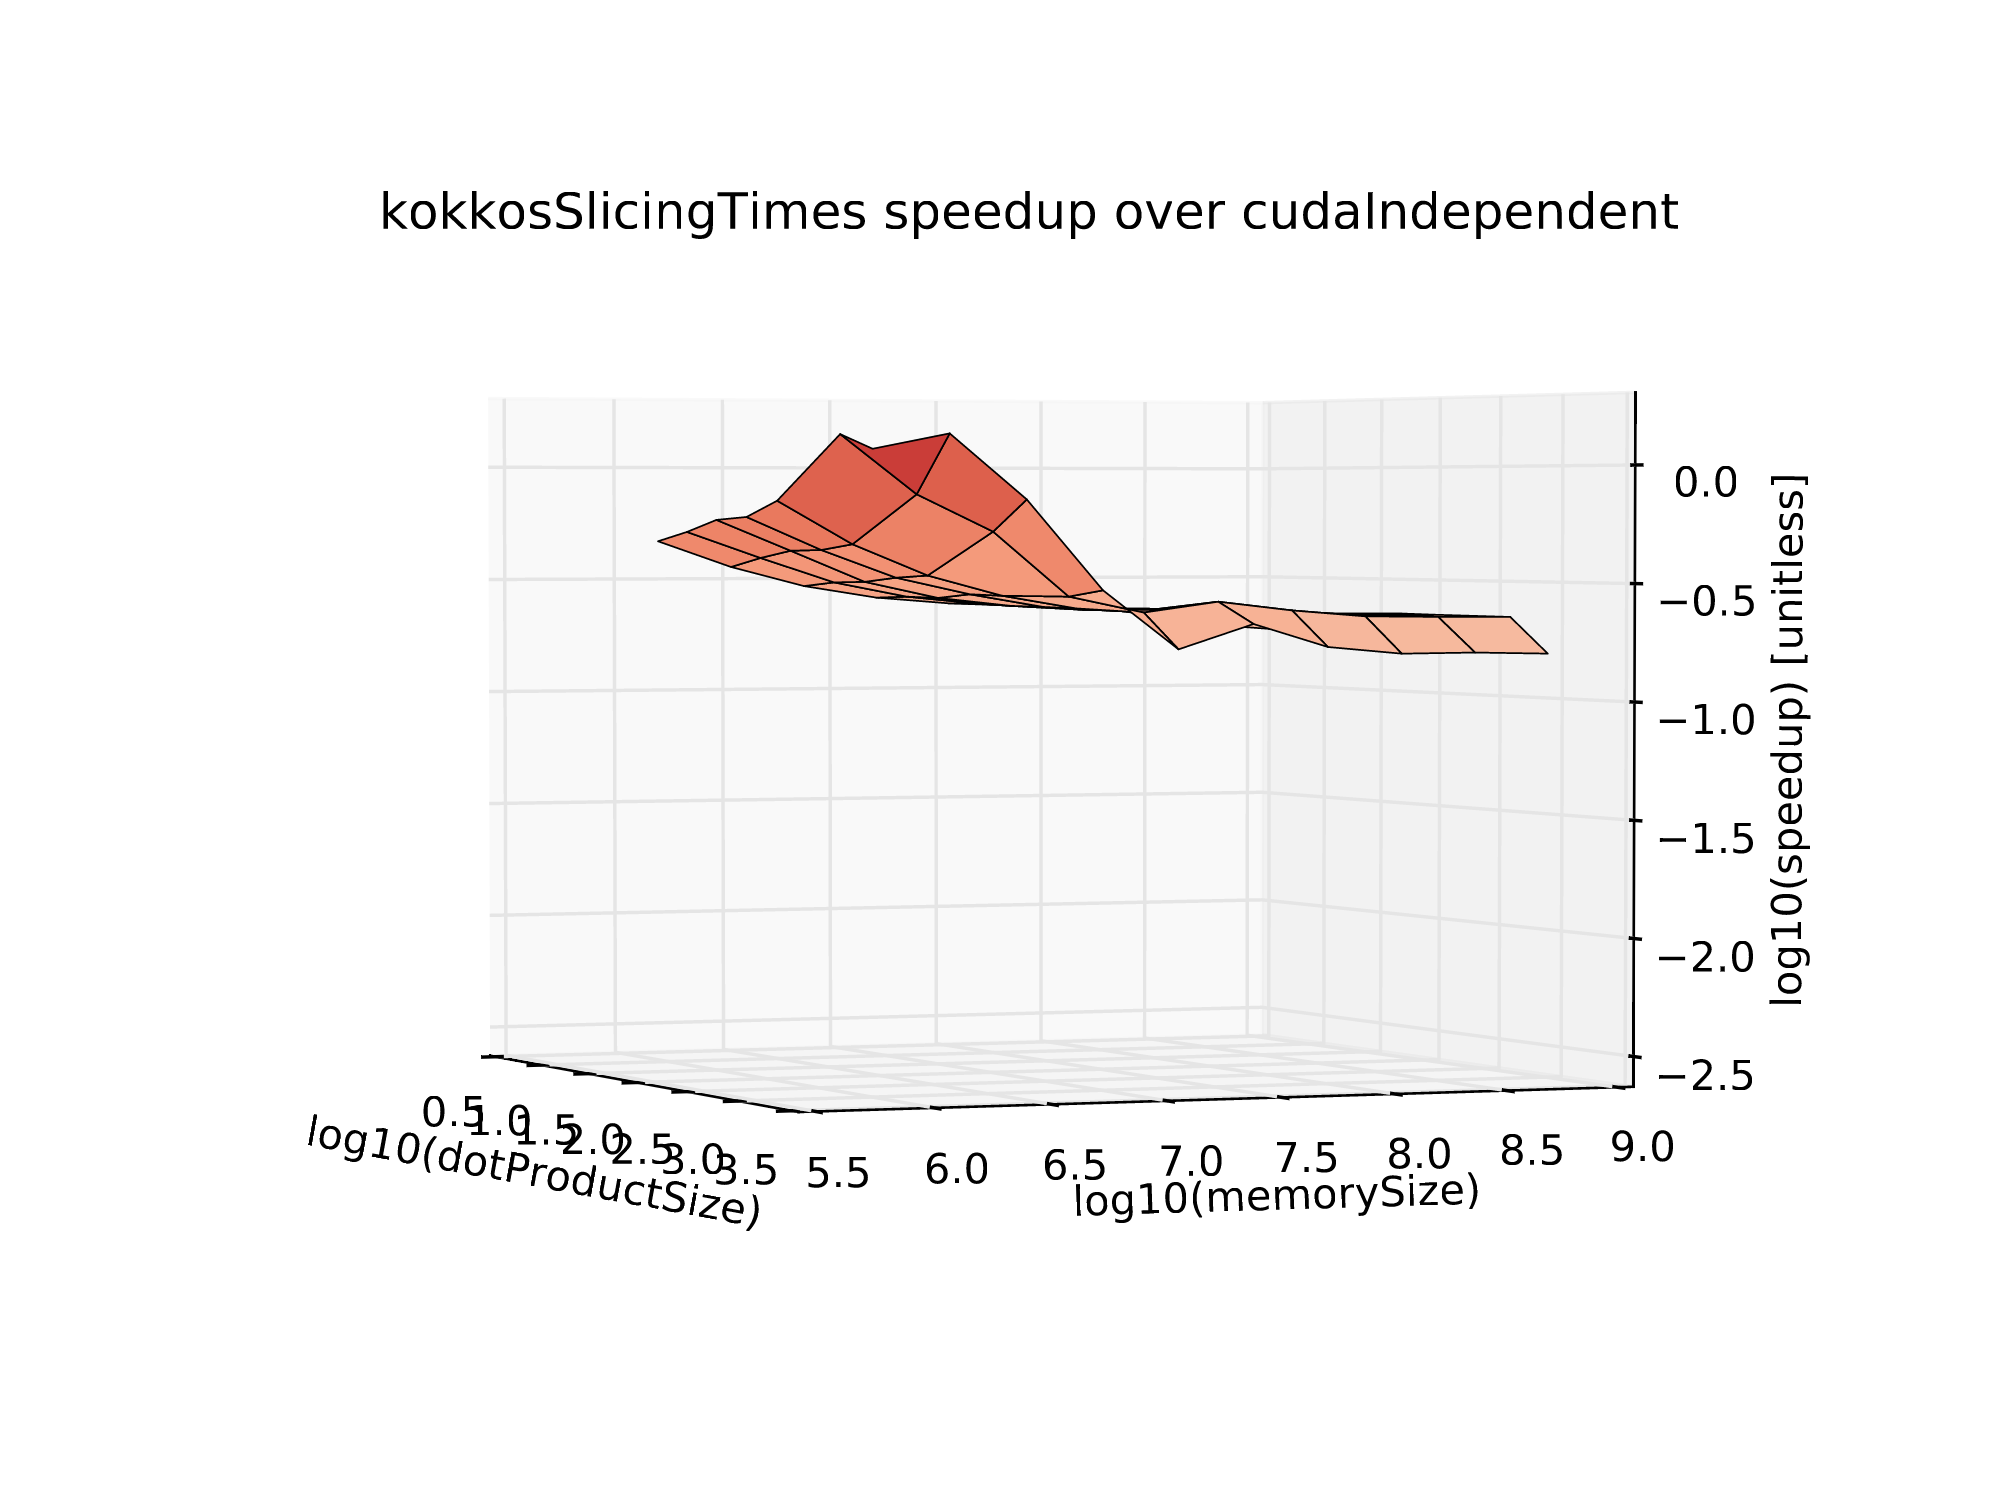
\includegraphics[scale = .17]{slicingvsindependent}

These results were generated by comparing independent algorithms to slicing on ContractFieldFieldScalar with $\ell = \mathcal{R} = 10, P = 8 - 1024$. We see that in the corner where the memory size is small and contraction size is small we get a small amount of speedup relative to independent Cuda code, which is promising. This is the corner where we would expect slicing to perform the best in comparison to independent parallelism, since in this corner flat parallelism is unable to fully saturate the GPU. The benefits of reuse in this corner are significant enough to outcompete flat parallelism. On the rest of the graph, however, the inability of slicing to saturate the GPU means that it is significantly slower that flat parallelism. Since $\ell = \mathcal{R} = 10$, the algorithm naturally only spawns 10 threads per block, which is not enough to produce good results. 

We're still working on an adaptive slicing implementation that can increase the size of a block and load more data into shared memory when necessary. That approach should benchmarked and included in the report by the end of this week! 

% Alex
\section{Tiling} \label{sec:tiling}

The final parallelization technique we used for these tensor contractions was tiling. This technique is similar to the tiled technique for matrix multiplication used in serial operations. Instead of relying on the cache to retain the relevant pieces of information, however, we use shared memory to explicitly store the data we care about. Once again, we will explain this algorithm by example. Consider one of the matrix multiplications in ContractFieldFieldScalar shown above. 

\begin{figure}
    \centering
    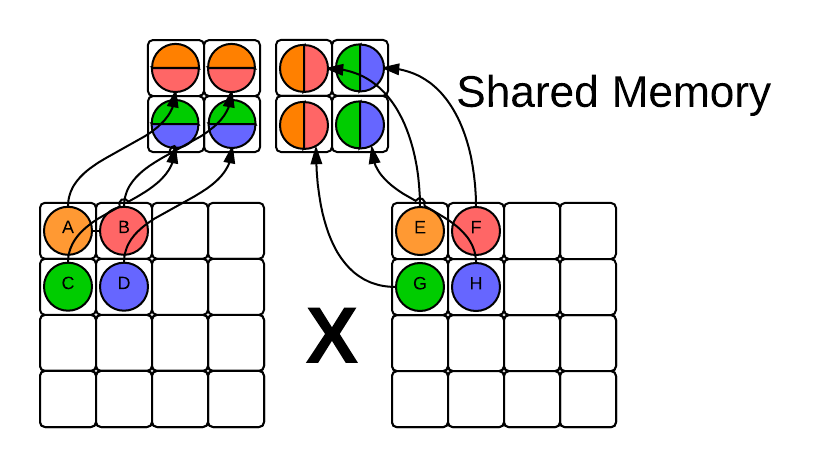
\includegraphics[scale = .7]{ContractFieldFieldScalarGraphicTiling}
    \caption{Demonstration of memory accesses for a tiling implementation of ContractFieldFieldScalar}
\end{figure}

For the sake of simplicity we'll consider a block to be four threads, which simplifies our computation since the matrix is four by four. On the left hand side, the block loads a four element tile into the shared memory of the threads. Once these elements are loaded into memory, each thread can begin computation of their element in the output matrix. Each thread computes as much of their output element as they can using the elements in shared memory, then we load a new tile into shared memory and continue the process, as shown below. We see that in this case we will have to load two tiles into shared memory before we have computed every output element in its entirety. 

\begin{figure}
    \centering
    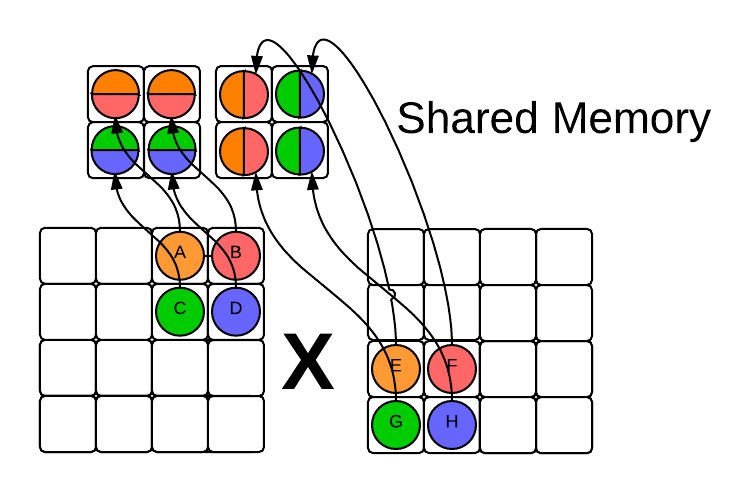
\includegraphics[scale = .7]{ContractFieldFieldScalarGraphicTiling2}
    \caption{Demonstration of memory accesses for a tiling implementation of ContractFieldFieldScalar}
\end{figure}

	Tiling can be viewed as a more specialized version of slicing, since they both use similar access patterns for shared memory. The difference between the two lies in tilings usage of multiple contractions per block, as well as the the distribution of a contractions operations over multiple loops of the routine. Because of these differences, tiling can routinely saturate the GPU in a way that pure slicing cannot, since the algorithm inherently limits the shared memory usage per block by reusing the same shared memory multiple times. Additionally, if we set the dimension of our tiles intelligently, we can reliably saturate the GPU with both blocks and threads, something that is very difficult to do adaptively with pure slicing. 
	
	Unfortunately, it is much less clear how exactly to tile in multiple dimensions. Unlike slicing, there seem to be multiple distinct ways of approaching the problem. One could create "tiles" with dimension equal to the contraction size, or any number less than the contraction dimension by unrolling the contraction to some intermediate degree. We haven't been able to fully explore every possibility in this area, and have simply treated the higher dimensional contractions as a fully unrolled contraction of one dimension. It is possible, however, that in some situations it would be more effective to create tiles with multiple degree. These tiles would have a different layout in memory who's efficiency would vary by situation. 
	
	Excerpts from our Cuda implementation of tiling are included below. The code assumes that tileSize (the horizontal and vertical dimensions of a tile) evenly divides both the contraction size and $\ell = \mathcal{R} = \text{numBasis}$.
	
\begin{figure}[H]
    \begin{lstlisting} [basicstyle=\tiny]
  extern __shared__ float tileStorage[];
  const unsigned int numbersPerTile = tileSize * tileSize;
  const unsigned int numberOfHorizontalTiles = contractionSize / tileSize;
  const unsigned int numberOfVerticalTiles = numBasis / tileSize;

  const unsigned int numberOfTiles = numCells * numberOfVerticalTiles * numberOfVerticalTiles;

  const unsigned int subRow = threadIdx.x / tileSize;
  const unsigned int subCol = threadIdx.x  - subRow * tileSize;

  unsigned int resultTileIndex = blockIdx.x;

  unsigned int resultSubmatrixIndex = resultTileIndex % (numberOfVerticalTiles * numberOfVerticalTiles);
  unsigned int resultMatrix = resultTileIndex / (numberOfVerticalTiles * numberOfVerticalTiles);

  // for tileNumber in 0...numberOfTilesPerSide
  for (unsigned int tileNumber = 0; tileNumber < numberOfHorizontalTiles; ++tileNumber) {
      
      // calculate result tile indices
      const unsigned int resultTileRow = resultSubmatrixIndex / numberOfHorizontalTiles;
      const unsigned int resultTileCol = resultSubmatrixIndex  -
        resultTileRow * numberOfHorizontalTiles;

      // calculate this threads actual output index
      const unsigned int row = resultTileRow * tileSize + subRow;
      const unsigned int col = resultTileCol * tileSize + subCol;

      // these are base indices into the shared memory
      const unsigned int leftBaseIndex = subRow * tileSize;
      const unsigned int rightBaseIndex = numbersPerTile + subCol;

      const unsigned int resultIndex = row * numBasis + col;

      // load the left and right tiles into shared memory
      syncthreads();
      tileStorage[threadIdx.x] = dev_contractionData_Left[resultMatrix * numBasis * contractionSize
        + row * contractionSize + tileNumber * tileSize + subCol];
      tileStorage[threadIdx.x + blockDim.x] = dev_contractionData_Right[resultMatrix * numBasis * contractionSize
        + (tileNumber * tileSize + subRow) * numBasis + col];
      
      // make sure everyone's finished loading their pieces of the tiles
      syncthreads();
      double sum = 0;
      for (unsigned int dummy = 0; dummy < tileSize; ++dummy) {
        sum +=
          tileStorage[leftBaseIndex + dummy] *
          tileStorage[rightBaseIndex + dummy * tileSize];
      }
      dev_contractionResults[resultIndex] += sum;
    }

 \end{lstlisting}
\end{figure}


Thus far in our research, we have found tiling to be the most effective algorithm for realizing parallel speedup. 

\begin{figure}[H]
    \centering
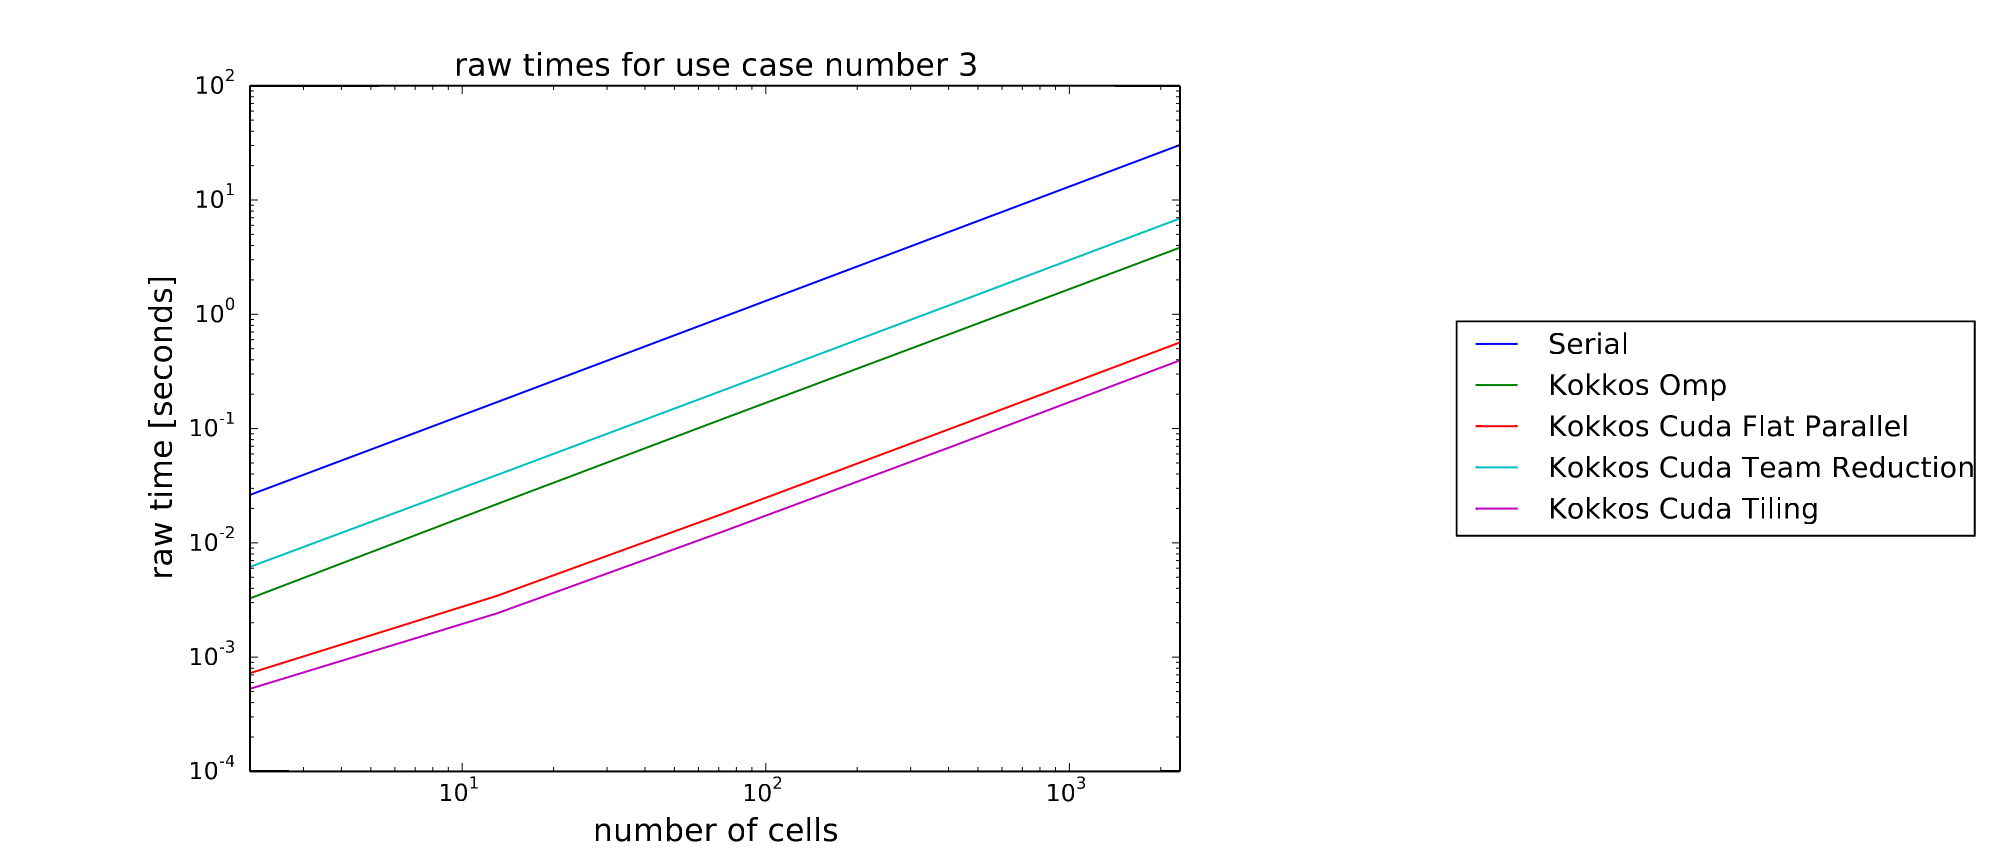
\includegraphics[scale = .2]{tilinguc1}
\caption{Raw times for many different algorithms used for ContractFieldFieldScalar. Note that Tiling is the best performing (lowest). This data was generated with $\ell=\mathcal{R}=125$, $p=216$}
\end{figure}
Consider the graph generated above for ContractFieldFieldScalar. We see that Tiling outperforms both flat parallelism and team reductions across the board. This trend continues for smaller use cases as well, as shown below when $\ell = \mathcal{R} = 8$, $P = 8$.

\begin{figure}[H]
    \centering
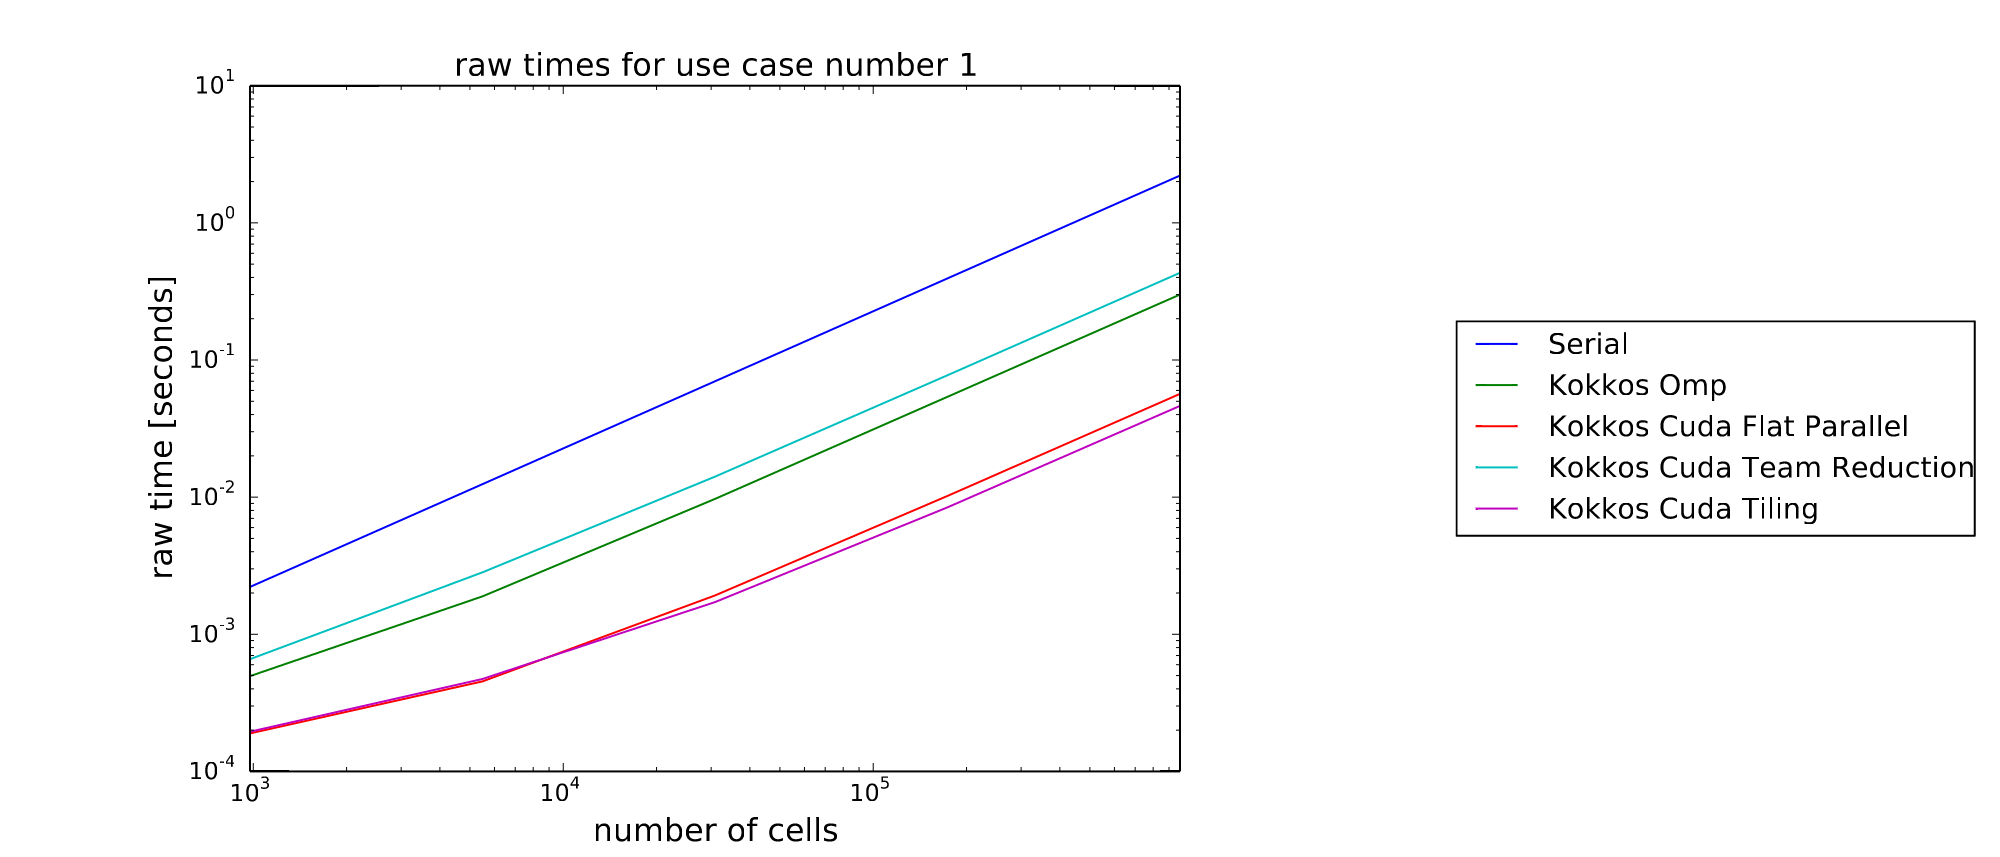
\includegraphics[scale = .2]{tilinguc2}
\caption{Raw times for many different algorithms used for ContractFieldFieldScalar. This data was generated with $\ell=\mathcal{R}=8$, $p=8$}
\end{figure}

In general, we have found that 2D tiling is the most effective method for achieving parallel speedup on these kernels. Initially, we were concerned that it would not perform as well on higher dimensionality kernels, where the size of the contraction is often \textit{much} larger than the number of basis functions. For example, consider the ContractFieldFieldTensor kernel, which can be described as $L_{C,\ell,P,d_1,d_2} \times R_{C, \mathcal{R}, P,d_1,d_2} = O_{C,\ell, \mathcal{R}}$. In essence, the kernel represents a series of three dimensional dot products. For this kernel, common use cases set $d_1$ and $d_2$ to $3$, with $p, \ell, \mathcal{R}$ ranging from $10$ to $100$. In these cases, the size of the contraction will often be larger than the number of basis functions by as much as an order of magnitude. This makes tiling significantly less efficient, since the number of blocks capable of working on a contraction using the tiling algorithm is given by $\frac{\text{number of basis functions}}{\text{size of a tile}}$. However, in these use cases, we found that tiling can still perform well as shown by the images below: 

\begin{figure}[H]
    \centering
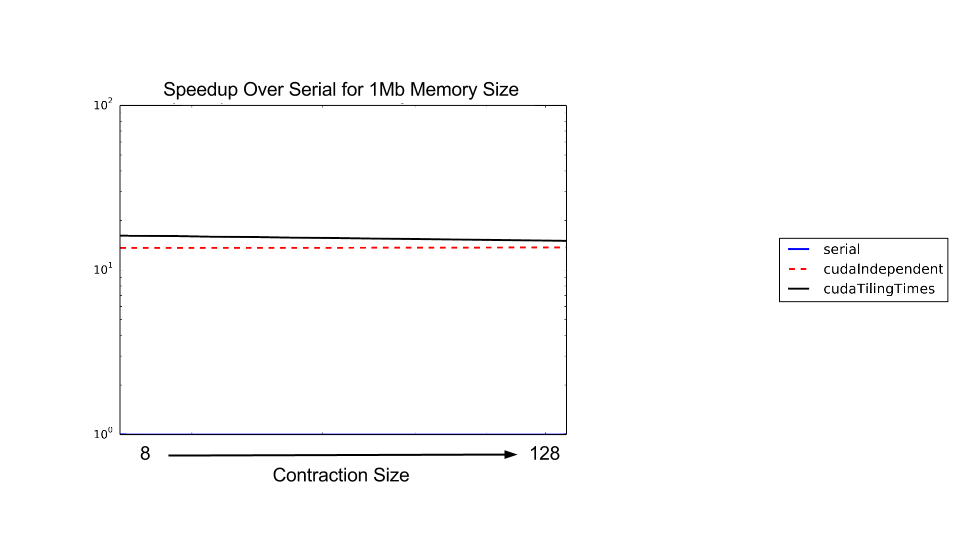
\includegraphics[scale = .2]{CFFTTiling1}
\caption{Raw times for serial, independent, and tiling approaches to ContractFieldFieldScalar. This data was generated with $\ell=\mathcal{R}=16$, $d_1=d_2=4$, with $p$ varying from $8$ to $128$. This graph uses a relatively low memory size, which limits the number of cells}
\end{figure}

\begin{figure}[H]
    \centering
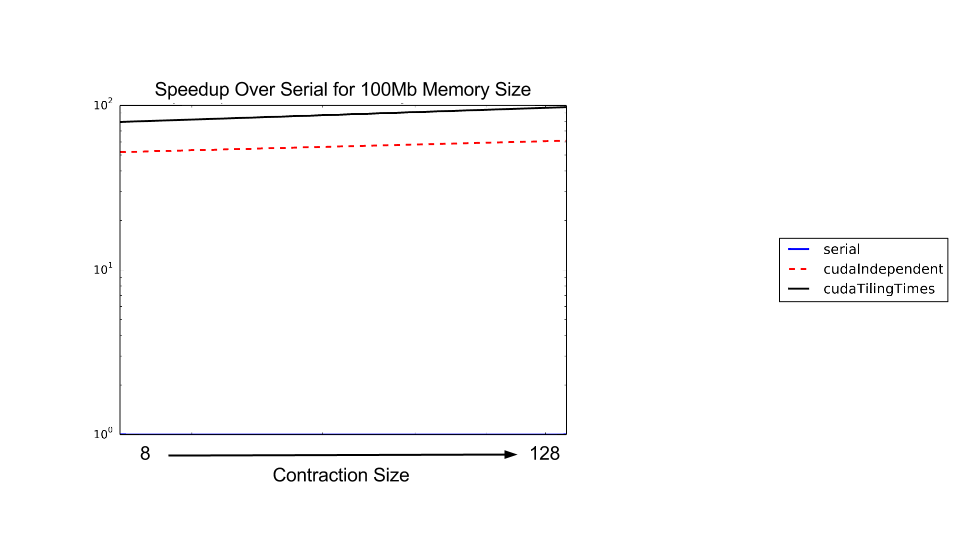
\includegraphics[scale = .2]{CFFTTiling2}
\caption{Raw times for serial, independent, and tiling approaches to ContractFieldFieldScalar. This data was generated with $\ell=\mathcal{R}=16$, $d_1=d_2=4$, with $p$ varying from $8$ to $128$. This data was collected while simulating a memory size an order of magnitude larger than the previous image, leading to a significantly higher cell count. }
\end{figure}
 
